\section{Preliminaries}
\label{sec:prelim}

\subsection{Routability Problem Formulation}
The key objective of routing is to maximize routability of the design, which is the quality of routing the circuit subject to net and design constraints.
The routing problem can be formulated as follows:
\begin{subequations}
\begin{align*}
    \max  \       & f(X), \\
    \text{s.t.}~~ & d(X) \leq 0, \\
                  & n(X) \leq 0.
\end{align*}
\end{subequations}
Here the constraints are categorised into two classes, network constraints $n(X)$ and design constraints $d(X)$. Network constraints indicate that the topology of the network must satisfy certain requirements, for example, pins of each net has to be all connected without loops formed. Design constraints, on the other hand, state that the implementation of the network topology is legal, such as no overlapping routes, routing direction follows the layer specifications. Our research fits within the routability optimisation problem. In particular, we are minimising the net constraint of congestion.

\subsection{Grid Model}
\label{subsec:grid model}

\begin{figure}[tb!]
    \centering
    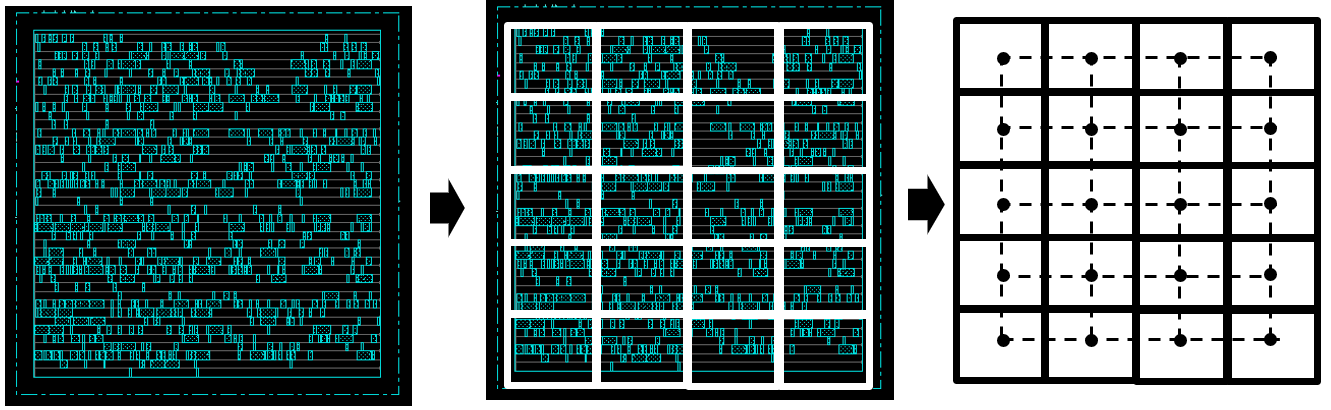
\includegraphics[width=3in]{grid_model}
	\caption{Design is divided into rectangular tiles (solid lines). The dark
		circles and dashed lines represent the vertices and the edges of the grid graph, respectively.}
	\label{fig:grid_model}
\end{figure}

Global routing is performed on a grid which is the logic graph representation of the physical chip. The grid graph \emph{G} is tile-based, which means that the entire chip is partitioned into multiple sub-regions, as illustrated in Fig.~\ref{fig:grid_model}. Each sub-region is called grid cell, or global routing cell. The cells are further gridded with vertical and horizontal gridlines, referred to as routing tracks, along which routes are determined and wires can be created. Each vertex in \emph{G} represents a corresponding tile, and each edge in \emph{G} between vertices corresponds to the shared boundary of two tiles.

\subsection{Routing Metrics for Network Constraints}
\subsubsection{Routing Capacity}
The graph \emph{G} used for global routing needs to capture the capacities of the routing regions. The capacity of an edge \emph{e} $\in$ \emph{G} between two vertices \emph{u} and \emph{v} is defined as the maximum number of available routing tracks between the routing regions of \emph{u} and \emph{v}. 

High precision capacity metric can be complex and possible in practice, such simple track-based capacity can be extended  to consider specific routing elements such as blockages, vias and pins.
\subsubsection{Congestion}
If the total usage of one edge is larger than its capacity, then the tile containing that edge is congested, the value is defined as $c(e)=\text{usage}(e)/\text{capacity}(e)$. Detailed routing will not be able to route all nets assigned to congested areas due to lack of routing resources. However, it is in some degree tolerable to the detailed router as it can spread the wires from the congested tiles to adjacent less-congested tiles, if there are any.
\subsubsection{Overflow}
Similar to congestion, when the usage of a tile is greater than its capacity, the amount of overhead is called overflow, $of(e)=\text{usage}(e)-\text{capacity}(e)$.
% \subsubsection{Wirelength}
% The minimization of wirelength is another important metric for global routing. Decreased wirelength implies smaller power consumption and delays, which are two key factors for  performance-driven optimization. Inherently, congestion minimization conflicts with wirelength minimization, because detours may be introduced to avoid congested regions and that leads to longer wirelength. Therefore, the trade-off between these features has to be carefully tuned based on the requirements of circuit design. 

\subsection{Supervised Data Learning Technique}
Data-learning is a powerful technique which can drive knowledge from big data, predict and generalise unseen data pattern. There are four main categories: Supervised, Unsupervised, Semi-supervised, and reinforcement learning. In the research field of physical design algorithms, supervised learning is widely used.

As is illustrated in Fig.~\ref{fig:ml_flow}, given certain features as the input, the training process builds a set of models, which will then be evaluated. One way of testing the quality of models is by feeding the same input features as were fed during training to see if predicted values are close enough to the original target output. After the evaluation, acceptable models are selected based on different purposes to make predictions and decisions for various applications. 
\begin{figure}[tb!]
    \centering
    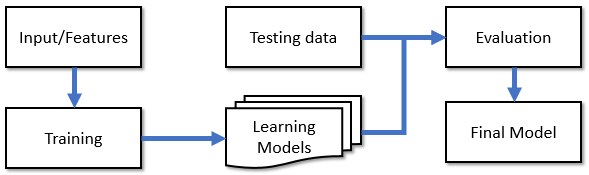
\includegraphics[width=.68\linewidth]{ML_flow}
    \caption{Supervised learning flow.}
    \label{fig:ml_flow}
\end{figure}
There are two types of applications fall under this \textit{ML} category:
\begin{itemize}
\item Regression. Given input to predict continuous values. For example, guess the height of one individual human based on one's age. 
\item Classification. The goal is to predict discrete values. Determine if an email is spam or not, a human is female or male. 
\end{itemize}

Examples of supervised learning algorithms include, decision trees, linear regression, support vector machines, neural networks, Multivariate Adaptive regression Splines.
